%% Copyright 2018 H.\ Rabus
%
% This work may be distributed and/or modified under the
% conditions of the LaTeX Project Public License, either version 1.3
% of this license or (at your option) any later version.
% The latest version of this license is in
%   http://www.latex-project.org/lppl.txt
% and version 1.3 or later is part of all distributions of LaTeX
% version 2005/12/01 or later.
%
% This work has the LPPL maintenance status `author-maintained'.
%
% This work consists of the file texbsp.tex
%

\documentclass[smallheadings]{scrartcl}

%%% GENERAL PACKAGES %%%%%%%%%%%%%%%%%%%%%%%%%%%%%%%%%%%%%%%%%%%%%%%%%%%%%%%%%%
% inputenc allows the usage of non-ascii characters in the LaTeX source code
\usepackage[utf8]{inputenc}
\usepackage{graphicx} 
\usepackage{float}
%\graphicspath{ {/u/hnatiuka/Praktikum/PPI/} }



% title of the document
\title{Bericht zu Serie 3}
% optional subtitle
%\subtitle{Draft from~\today}
% information about the author
\author{%
  Arsen Hnatiuk,\\%
  Max Huneshagen 
}
\date{\today} 


%%% LANGUAGE %%%%%%%%%%%%%%%%%%%%%%%%%%%%%%%%%%%%%%%%%%%%%%%%%%%%%%%%%%%%%%%%%%
% babel provides hyphenation patterns and translations of keywords like 'table
% of contents'
\usepackage[ngerman]{babel}

%%% HYPERLINKS %%%%%%%%%%%%%%%%%%%%%%%%%%%%%%%%%%%%%%%%%%%%%%%%%%%%%%%%%%%%%%%%
% automatic generation of hyperlinks for references and URIs
\usepackage{hyperref}

%%% MATH %%%%%%%%%%%%%%%%%%%%%%%%%%%%%%%%%%%%%%%%%%%%%%%%%%%%%%%%%%%%%%%%%%%%%%
% amsmath provides commands for type-setting mathematical formulas
\usepackage{amsmath}
\numberwithin{equation}{section}
% amssymb provides additional symbols
\usepackage{amssymb}
% HINT
% Use http://detexify.kirelabs.org/classify.html to find unknown symbols!

%%% COLORS %%%%%%%%%%%%%%%%%%%%%%%%%%%%%%%%%%%%%%%%%%%%%%%%%%%%%%%%%%%%%%%%%%%%
% define own colors and use colored text
\usepackage[pdftex,svgnames,hyperref]{xcolor}

%%% Code Listings %%%%%%%%%%%%%%%%
% provides commands for including code (python, latex, ...)
\usepackage{listings}
\definecolor{keywords}{RGB}{255,0,90}
\definecolor{comments}{RGB}{0,0,113}
\definecolor{red}{RGB}{160,0,0}
\definecolor{green}{RGB}{0,150,0}
\lstset{language=Python, 
        basicstyle=\ttfamily\small, 
        keywordstyle=\color{keywords},
        commentstyle=\color{comments},
        stringstyle=\color{red},
        showstringspaces=false,
        identifierstyle=\color{green},
        }


\usepackage{paralist}
\usepackage{nicefrac}
% setting the font style for input und returns in description items
\newcommand{\initem}[2]{\item[\hspace{0.5em} {\normalfont\ttfamily{#1}} {\normalfont\itshape{(#2)}}]}
\newcommand{\outitem}[1]{\item[\hspace{0.5em} \normalfont\itshape{(#1)}]}
\newcommand{\bfpara}[1]{
	
	\noindent \textbf{#1:}\,}

\usepackage{MnSymbol}
\begin{document}

% generating the title page
\maketitle
% generating the table of contents (requires to run pdflatex twice!)
\tableofcontents
\bigskip

\hrule
\hrule

%%% BEGIN OF CONTENT %%%%%%%%%%%%%%%%%%%%%%%%%%%%%%%%%%%%%%%%%%%%%%%%%%%%%%%%%%

\section{Einleitung}

Die in dieser Serie implementierten Programme ermöglichen die numerische Lösung des in Serie 2 betrachteten Gleichungssystems
\begin{align}
A^{(d)}\hat{u} = b
\label{eq:glc}
\end{align}
wobei $A^{(d)}$ eine Bandmatrix der Dimension $d$ und $\hat{u}$ eine Approximation der Lösung $u$ der Laplace Gleichung ist. $b$ ist der Vektor der Randbedingungen und der Werte der in der Laplace Gleichung gegebenen Funktion $f$ auf den in Serie 2 ausgewählten Punkten. Die Lösung wird durch LU-Zerlegung der Bandmatrix und durch Rückwärtssubstitution gewonnen.

Die Programme erlauben auch eine Untersuchung der Eigenschaften von Band- und Hilbertmatrizen, wie zum Beispiel die Berechnung der Kondition.

\section{Theorie}

\subsection{Laplace Gleichung}
Die Lösung des Systems \ref{eq:glc} erfolgt durch die LU-Zerlegung der $A^{(d)}$ Matrix. Wir können also $TA^{(d)}=LU$ für eine Permutationsmatrix $P$, eine unipotente untere Dreiecksmatrix $L$ und eine invertierbare obere Dreiecksmatrix $U$ schreiben. Dann lässt sich die Gleichung \ref{eq:glc} so darstellen:
\begin{align}
	T^tLU\hat{u}=b
	\label{eq:lu}
\end{align}
Man gewinnt die Werte von $\hat{u}$, indem man mittels Rückwärtssubstitution die Gleichung 
\begin{align}
	T^tLz=b
	\label{eq:lu1}
\end{align}
für ein $z\in \mathbb{R}^{(n-1)^d}$ löst. Dies ist möglich, weil $L$ eine Dreiecksmatrix mit Einsen auf der Hauptdiagonale ist. Die Werte von $\hat{u}$ rechnet man durch Rückwärtssubstitution in der Gleichung \eqref{eq:lu2} aus. Dies ist möglich, weil alle Hauptdiagonaleinträge von $R$ nach Numerische Lineare Algebra ungleich $0$ sind (dies sind die sogenannten Pivotelemente).
\begin{align}
	R\hat{u}=z
	\label{eq:lu2}
\end{align}
Wenn man die Gleichungen \eqref{eq:lu1} und \eqref{eq:lu2} zusammensetzt, so erhält man \eqref{eq:lu}.

Aus der numerischen linearen Algebra wissen wir, dass die LU-Zerlegung einer Bandmatrix der ersten Dimension und Feinheit $n$ eine höhere Anzahl von nicht-null Einträgen besitzt, als die Bandmatrix selbst. Und zwar, während nur die Hauptdiagonale und die zwei Nebendiagonalen (also $n+2(n-1)$-viele Einträge) der Bandmatrix besetzt sind, sind jeweils die Hauptdiagonale und eine Nebendiagonale von der L und U Matrizen besetzt (also $2n+2(n-1)$-viele Einträge).

Es gibt zwei Fehlerquellen für die numerische Lösung $\hat{u}$. Einerseits ist die Approximation der zweiten Ableitung von $u$ durch den Differentialquotienten aus Serie 1 nicht exakt und hat einen absoluten Fehler der Ordnung $\mathcal{O}(\frac{1}{n^2})$, wobei $n$ die Feinheit der Diskretisierung des Definitionesbereichs ist. Andererseits ist die Berechnung der Lösung mittels LU-Zerlegung und Rückwärtssubstitution auf einem Rechner auch fehlerhaft. Nach der numerischen linearen Algebra lässt sich der absolute Rundungsfehler der Lösung für eine Bandmatrix $A$ wie folgt abschätzen \cite{nla}:
\begin{align}
\|u-\hat{u}\|_{\infty}\le \epsilon_{mach}&(1+\mathcal{O}(\epsilon_{mach}))(n+2)c_g\kappa(A)\|\hat{u}\|_{\infty} \\
\text{wobei } c_g&=1+3\sum_{k=1}^{n-1}\frac{\|M^{(k)}\|_{\infty}}{\|A\|_{\infty}}
\end{align}
In diesem Fall ist $M^{(k)}$ eine im Laufe der LU-Zerlegung duch Streichen von geeigneten Zeilen und Spalten von bestimmten Zwischenergebnis-Matrizen gewonnene Matrix.

\subsection{Hilbert-Matrizen}
Unsere Programme ermöglichen auch die Arbeit mit Hilbert-Matrizen. Diese dienen als Beispiel schlecht konditionierter Matrizen und sind wie folgt definiert:
\begin{align}
	H_m &:= (a_{ij})_{1\le i, j \le m} \in \mathbb{R}^{m\times m}, 	\\
	a_{ij} &:= \frac{1}{i+j-1} \label{eq:hb1}
\end{align}
Das Inverse einer Hilbert-Matrix ist wie folgt definiert:
\begin{align}
	H_m^{-1}& := (b_{ij})_{1\le i, j \le m} \in \mathbb{R}^{m\times m},	\\
	b_{ij} := \frac{(-1)^{i+j}}{i+j-1}\cdot &\frac{(m+i-1)!}{(i-1)!^2(m-i)!}\cdot \frac{(m+j-1)!}{(j-1)!^2(m-j)!}
\end{align}

Aus der numerischen linearen Algebra wissen wir, dass für die Kondition $\kappa$ einer Matrix $A$ gilt
\begin{align}
	\kappa(A)=\|A\|\cdot \|A^{-1}\|
\end{align}
Wenn wir die Spaltensummennorm $\|\cdot \|_{\infty}$ benutzen, ist die hohe Kondition einer Hilbert-Matrix leicht zu sehen. Aus \ref{eq:hb1}  sieht man, dass die erste Spalte von $H_m$ die höchste Spaltensumme hat, und es gilt
\begin{align}
	\|H_m\|_{\infty}=\sum_{i=1}^{m}\frac{1}{i}
\end{align}
Diese Reihe divergiert. Die Einträge von $H_m^{-1}$ sind dabei sehr groß. Schon für $i=j=1$ gilt $b_{ij} = m^2$, also die Norm von dieser Matrix wächst mindestens quadratisch. Folglich ist die Kondition $\kappa(H_m)\gg1$ für $m>1$.

<<<<<<< HEAD

\section{Experimente}

\subsection{Numerische Lösung}

In dieser Aufgabe ist die Laplace-Gleichung mit der exakten Lösung $u(x)=\prod_{j=1}^{d}x_j(1-x_j)$ auf dem Bereich $[0, 1]^d$ numerisch zu lösen, wobei $d$ die Dimension des Systems ist. Offensichtlich ist $u$ auf dem Rand von $[0, 1]^d$ die Nullabbildung, also sind alle Randdaten Null. Der Vektor $b$ aus \ref{eq:glc} besteht also nach Serie 2 nur aus der zweiten Ableitung $f$ von $u$ ausgewertet auf den Punkten der in Serie 2 definierten Diskretisierung von $[0, 1]^d$. Es gilt für $d=1, 2, 3$ entsprechend:

\begin{align}
f_1(x)&=2 \\
f_2(x) = 2(x_1(1-x_1)&+x_2(1-x_2)) \\
f_3(x)= 2(x_1(1-x_1)x_2(1-x_2)+x_1(1-x_1)&x_3(1-x_3)+x_2(1-x_2)x_3(1-x_3))
\end{align}
Mit der bekannten Funktion $f$ lässt sich das System mittels der Implementierung aus Teil 1 lösen. Zu einer gegebenen Dimension und Feinheit der Diskretisierung erstellt das Programm den Vektor $b$ und löst das Gleichungssystem. Da die exakte Lösung auch bekannt ist, lässt sich diese mit der numerischen Lösung vergleichen.

\begin{figure}
	\centering
	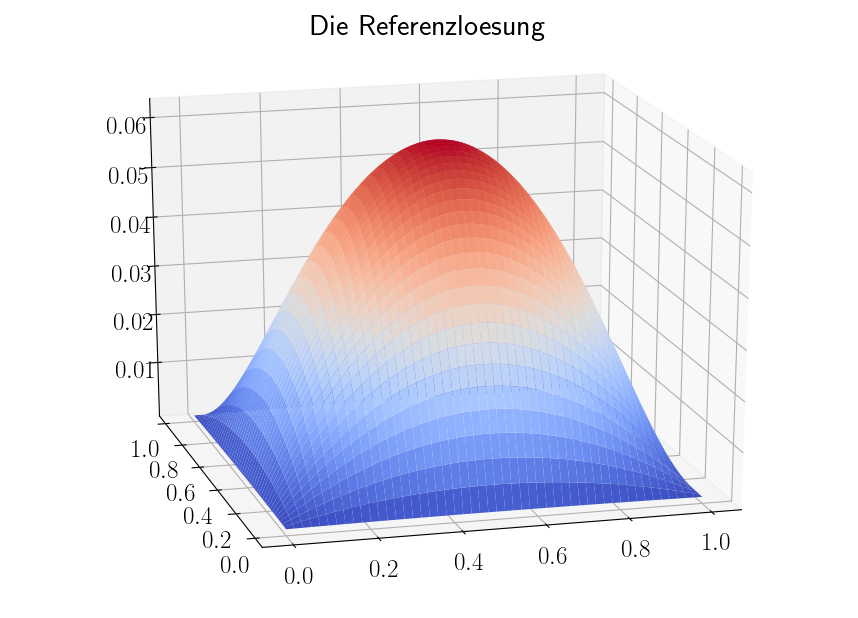
\includegraphics[width=0.7\linewidth]{Bericht/Bilder/referenz}
	\caption{Die exakte Lösung des Gleichungsystems}
	\label{fig:referenz}
\end{figure}

\begin{figure}
	\centering
	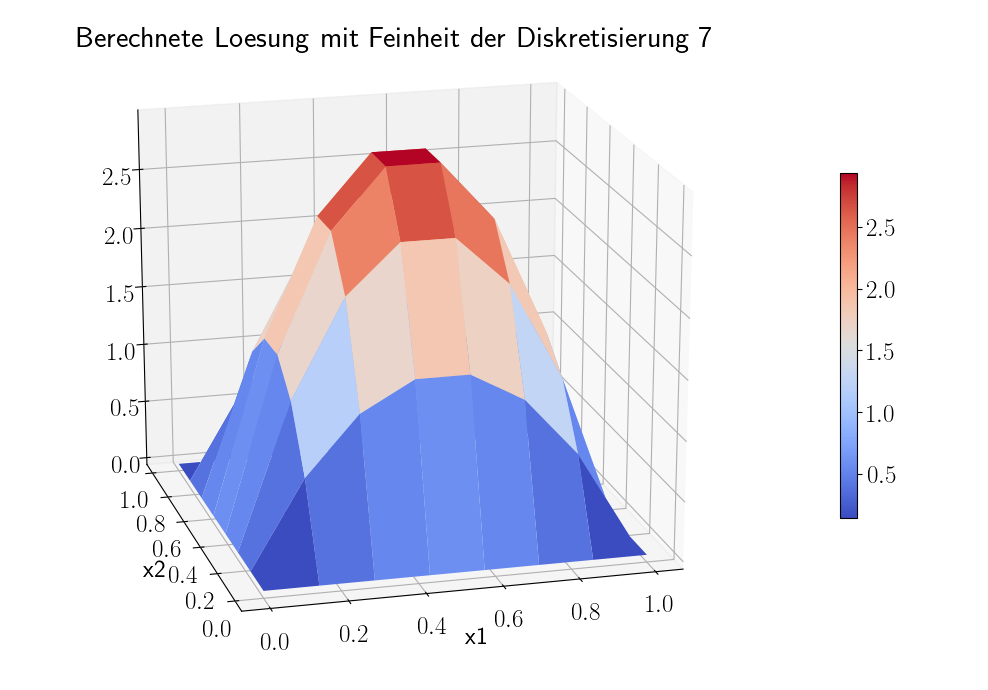
\includegraphics[width=0.7\linewidth]{Bericht/Bilder/3dlos7}
	\caption{Die numerishe Lösung mit Feinheit der Diskretisierung 7}
	\label{fig:3dlos7}
\end{figure}

\begin{figure}
	\centering
	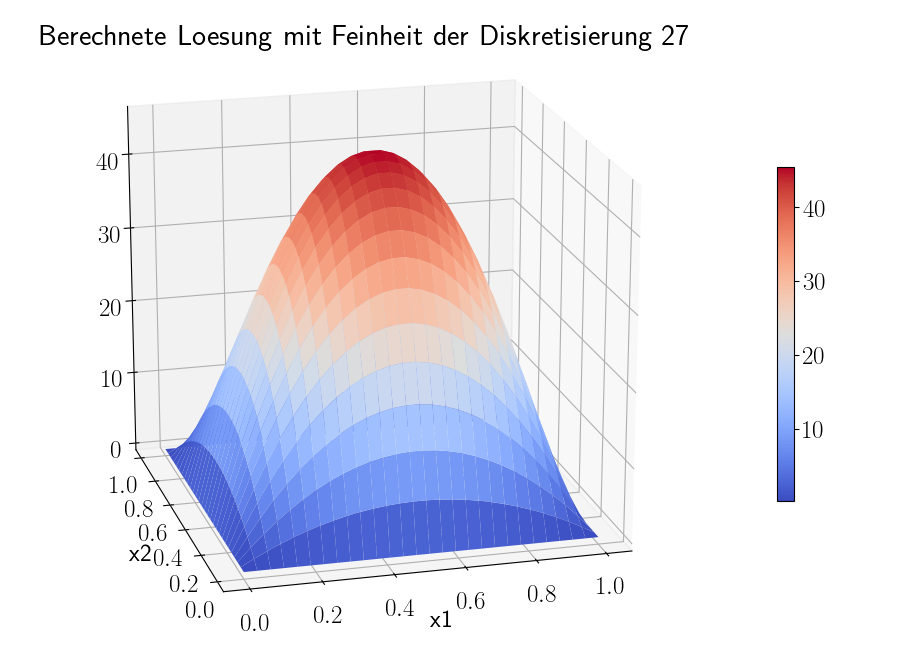
\includegraphics[width=0.7\linewidth]{Bericht/Bilder/3dlos27}
	\caption{Die numerishe Lösung mit Feinheit der Diskretisierung 27}
	\label{fig:3dlos27}
\end{figure}

Die Implementierung aus Teil 1 erlaubt eine grafische Darsetllung der Lösungen für den Fall $d=2$. Man sieht aus \ref{fig:referenz}, \ref{fig:3dlos7} und \ref{fig:3dlos27}, dass obwohl die numerische Lösungen die gleiche Gestalt wie die Referenzlösungen haben, nehmen diese viel größere Werte als die exakte Lösung an. Dieses Verhalten wird in \ref{fig:3dfel7} und \ref{fig:3dfel27} veranschaulicht. 

\begin{figure}
	\centering
	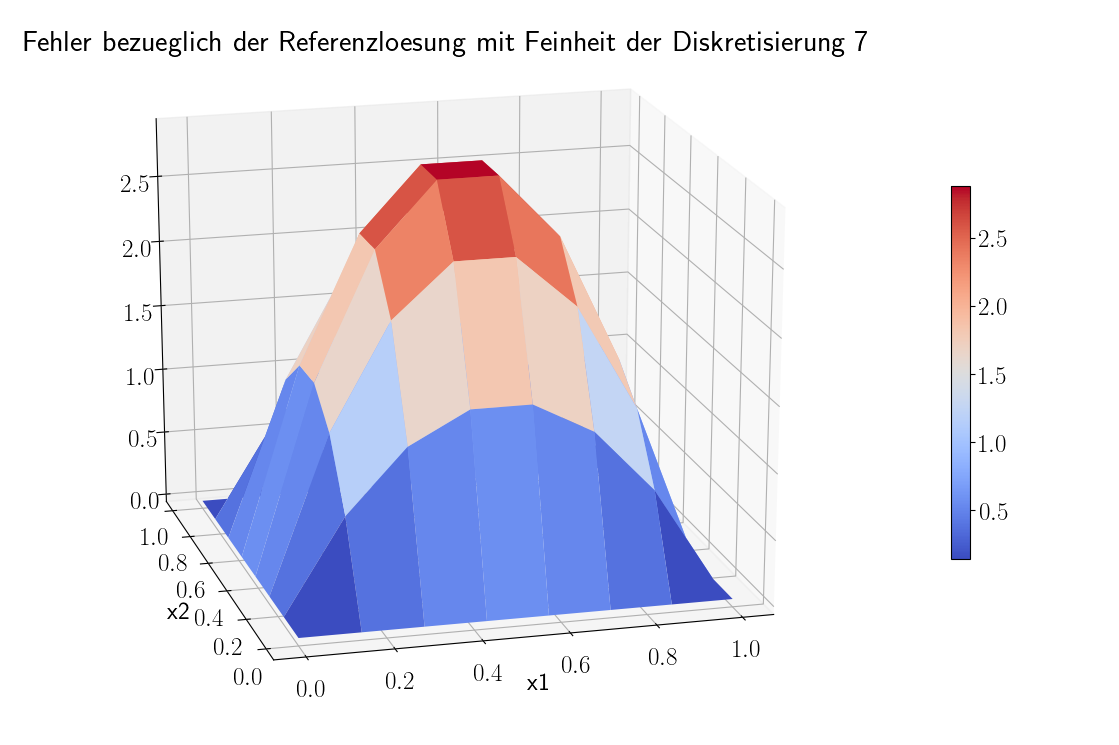
\includegraphics[width=0.7\linewidth]{Bericht/Bilder/3dfeh7}
	\caption{Der asolute Fehler der numerischen Lösung bezüglich der exakten Lösung mit Feinheit der Diskretisierung 7}
	\label{fig:3dfel7}
\end{figure}

\begin{figure}
	\centering
	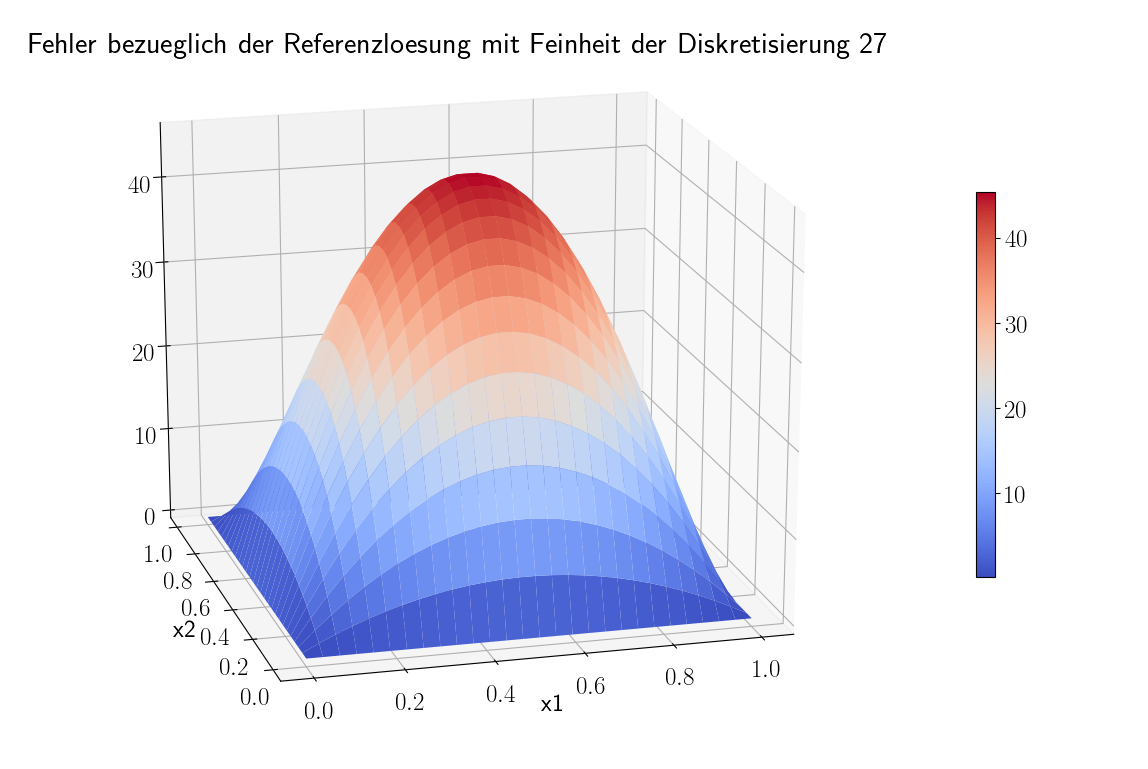
\includegraphics[width=0.7\linewidth]{Bericht/Bilder/3dfel27}
	\caption{Der asolute Fehler der numerischen Lösung bezüglich der exakten Lösung mit Feinheit der Diskretisierung 27}
	\label{fig:3dfel27}
\end{figure}

Diese Divergenz der numerischen Lösung von der exakten Lösung lässt sich in allen betrachteten Dimensionen beobachten, und der Fehler wächst in jedem Fall proportional zur Feinheit der Diskretisierung. Die Abbildungen \ref{fig:konvdim1}, \ref{fig:konvdim2} und \ref{fig:konvdim3} stellen dieses Verhalten grafisch dar.

\begin{figure}
	\centering
	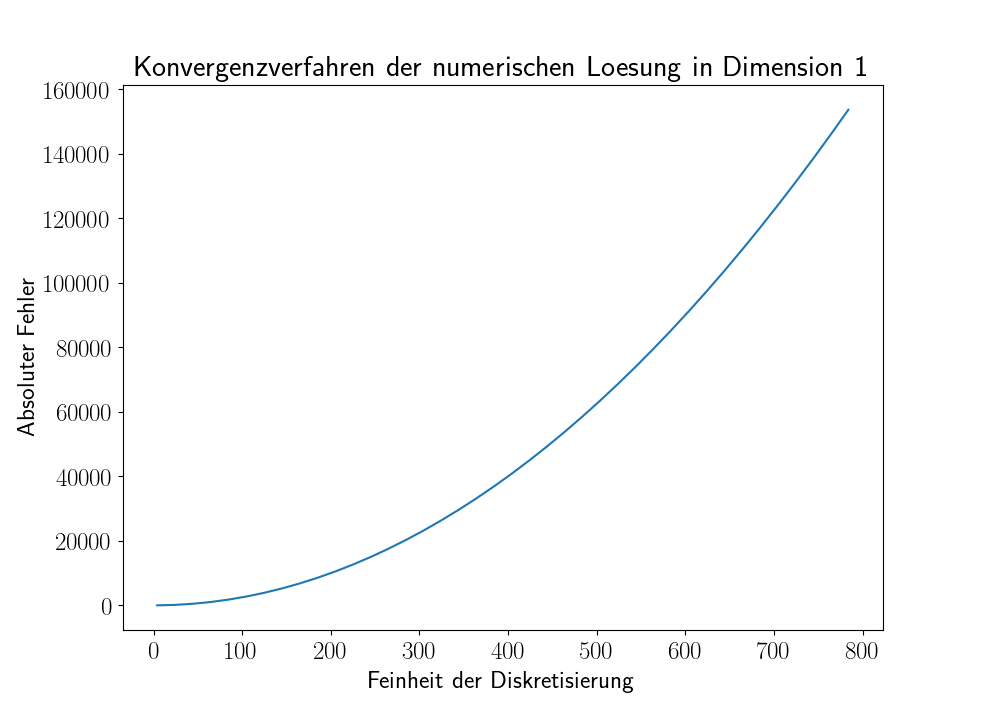
\includegraphics[width=0.7\linewidth]{Bericht/Bilder/konvdim1}
	\caption{Das Konvergenzverhalten der numerischen Lösung in Dimension 1}
	\label{fig:konvdim1}
\end{figure}

\begin{figure}
	\centering
	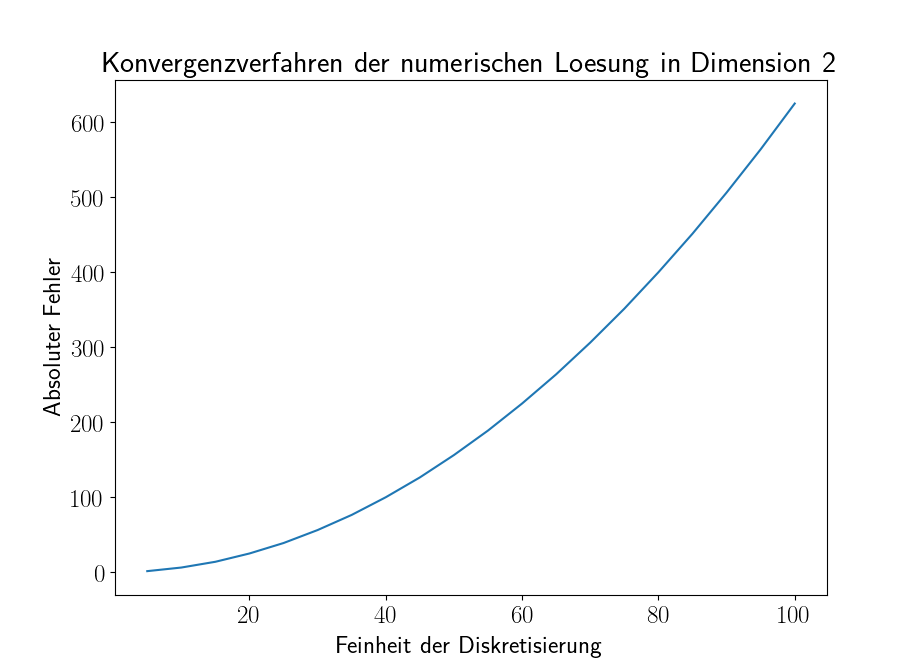
\includegraphics[width=0.7\linewidth]{Bericht/Bilder/konvdim2}
	\caption{Das Konvergenzverhalten der numerischen Lösung in Dimension 2}
	\label{fig:konvdim2}
\end{figure}

\begin{figure}
	\centering
	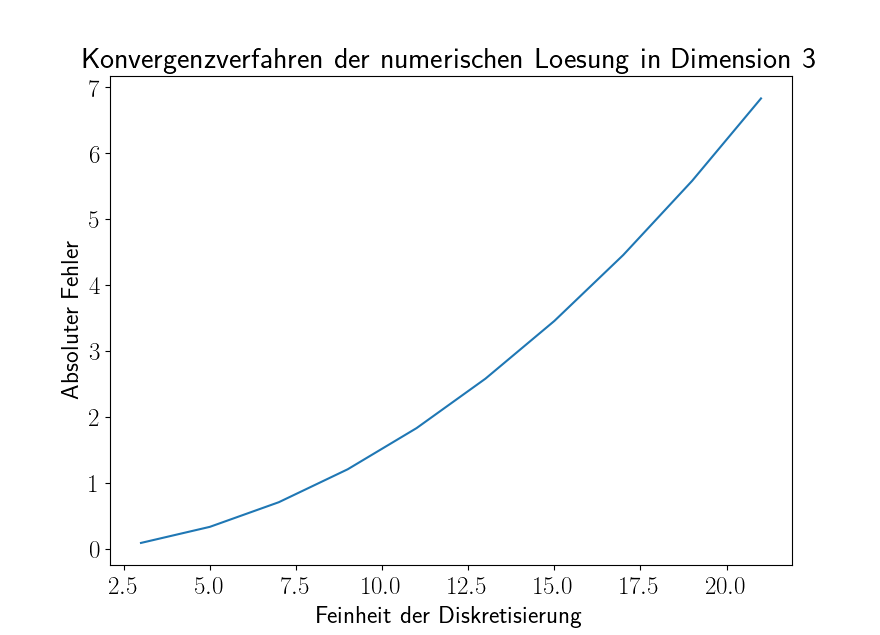
\includegraphics[width=0.7\linewidth]{Bericht/Bilder/konvdim3}
	\caption{Das Konvergenzverhalten der numerischen Lösung in Dimension 3}
	\label{fig:konvdim3}
\end{figure}

\subsection{Sparsity und Kondition}

\begin{figure}
	\centering
	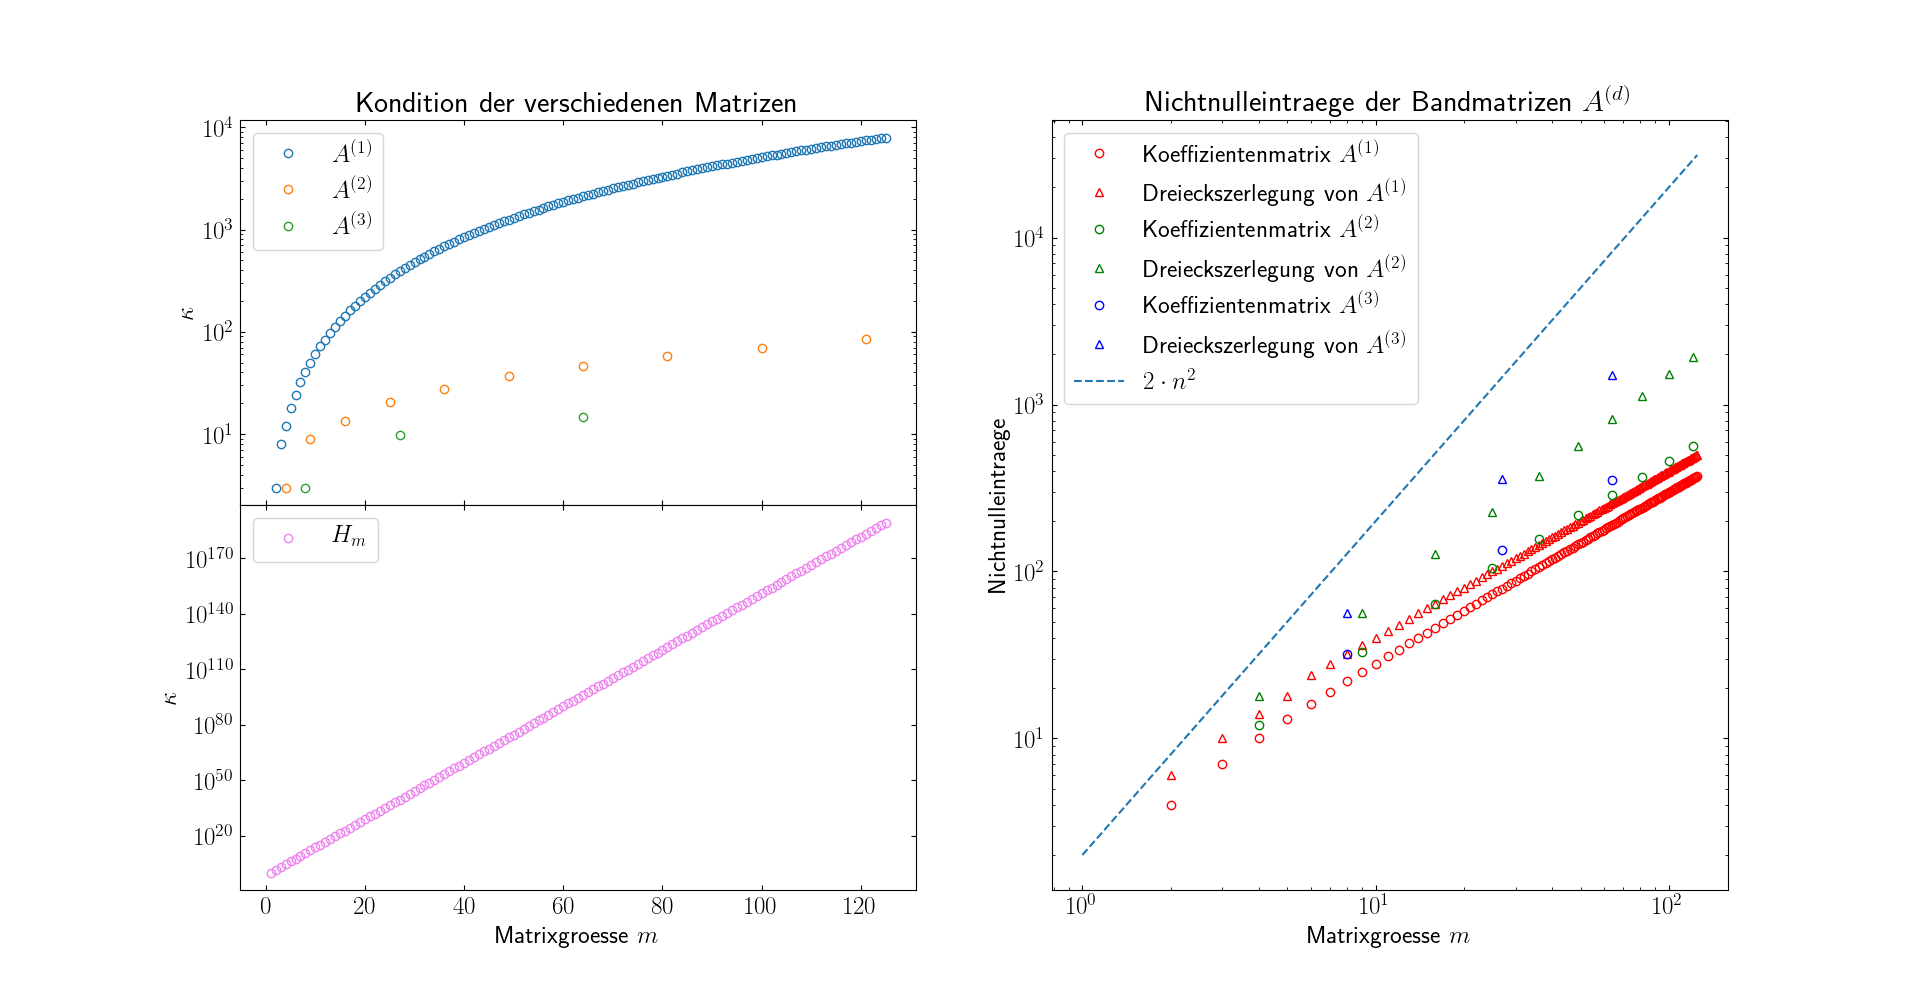
\includegraphics[width=\linewidth]{Bericht/Bilder/sparsekon}
	\caption{Die Kondition der betrachteten Matrizen und die Sparsity der LU Zerlegung}
	\label{fig:sparsekon}
\end{figure}

Die \textit{sparsity} der LU Zerlegung der Bandmatrizen lässt sich mittels der Implementierung aus Teil 1 Berechnen. In \ref{fig:sparsekon} sieht man, dass die Anzahl von nicht-null Einträgen in jeder Dimension bei der LU-Zerlegung höher ist, als bei der ursprünglichen Bandmatrix. Dies stimmt mit der Theorie überein, weil wir wissen, dass dies für den eindimensionalen Fall gelten muss. Im mehrdimensionalen Fall sind die bzgl. des eindimensionalen Falls zusätzliche Einträge in der Bandmatrix genau die 1-Einträge auf bestimmten Nebendiagonalen. Aus der Formel der Matrixmultiplikation folgt, dass es für jeden solchen Eintrag mindestens einen zusätzlichen nicht-null Eintrag in der L und/oder U Matrix gibt. Folglich muss es in jeder Dimension mehr nicht-null Einträgen in der LU-Zerlegung geben, als in der Bandmatrix.

Figur \ref{fig:sparsekon} zeigt auch, dass die Kondition der Bandmatrix in jeder Dimension proportional zur Feinheit der Diskretisierung wächst. Dies stimmt mit dem in der numerischen linearen Algebra berechneten Ergebnis überein. Die Spektralkondition einer eindimensionalen Bandmatrix der Feinheit 


\subsection{3.6}

Gemäß Aufgabe~3.6 der Aufgabenstellung wurde die Kondition der Hilbertmatrix $H_m$ in Abhängigkeit der Matrixgröße $m$ untersucht und graphisch dargestellt. Ebenso wurde das Gleichungssystem 
=======
\section{Theorie}

\subsection{Fehlerabschätzung mit Hilfe der Kondition}

Nach Bemerkung~4.4 des Skriptes \textit{Numerische Lineare Algebra} entspricht die Kondition $\kappa(A)$ einer Matrix $A$ der relativen Kondition des linearen Gleichungssystems $f(x)=b \iff Ax=b$. Nach Lemma~3.3 gilt für die Kondition von $f$:
\begin{align}
\lsem f(x+w)-f(x)\rsem &\leq \kappa(f;x)\lsem w\rsem + o(\lsem w \rsem)\text{,   } (\lsem w \rsem \rightarrow 0)\\
&\stackrel{.}{=} \kappa(f;x)\lsem w\rsem
\end{align}

\section{Experimente}

Gemäß Aufgabe~3.6 der Aufgabenstellung wurde die Kondition der Hilbertmatrix $H_m$ in Abhängigkeit der Matrixgröße $m$ experimentell untersucht und graphisch dargestellt. Ebenso wurde das Gleichungssystem 
\begin{align}
H_mx^{(i)}=e_i
\label{eq:hil_lgs}
\end{align}
für $m=2^k$, $k=0,1,2,\dots$ numerisch unter Ausnutzung der $L$-$U$-Zerlegung (s.~Schnittstellendoku) gelöst. Die aus den numerischen Verfahren gewonnene Lösung $\tilde{x}^{(i)}$ wurde mit der exakten Lösung $x^{(i)}$ verglichen. Letztere ergibt sich aus \eqref{eq:hil_lgs} als die $i$-te Spalte der inversen Hilbert-Matrix:
>>>>>>> f1a94ebf311269b8c67070ec269a586f14f907c6
\begin{align}
x^{(i)}=H_m^{-1}e_i\equiv(\text{$i$-te Spalte von }H_m^{-1}).
\end{align}
Die beiden Vektoren wurden anhand der Größe
\begin{align*}
\max\limits_{i=1,\dots,m}\|\tilde{x}^{(i)}-x^{(i)}\|_\infty
\end{align*}
verglichen. Das Ergebnis ist in Abb.~\ref{fig:hil_kond_fehl}
dargestellt.

\begin{figure}[H]
\centering
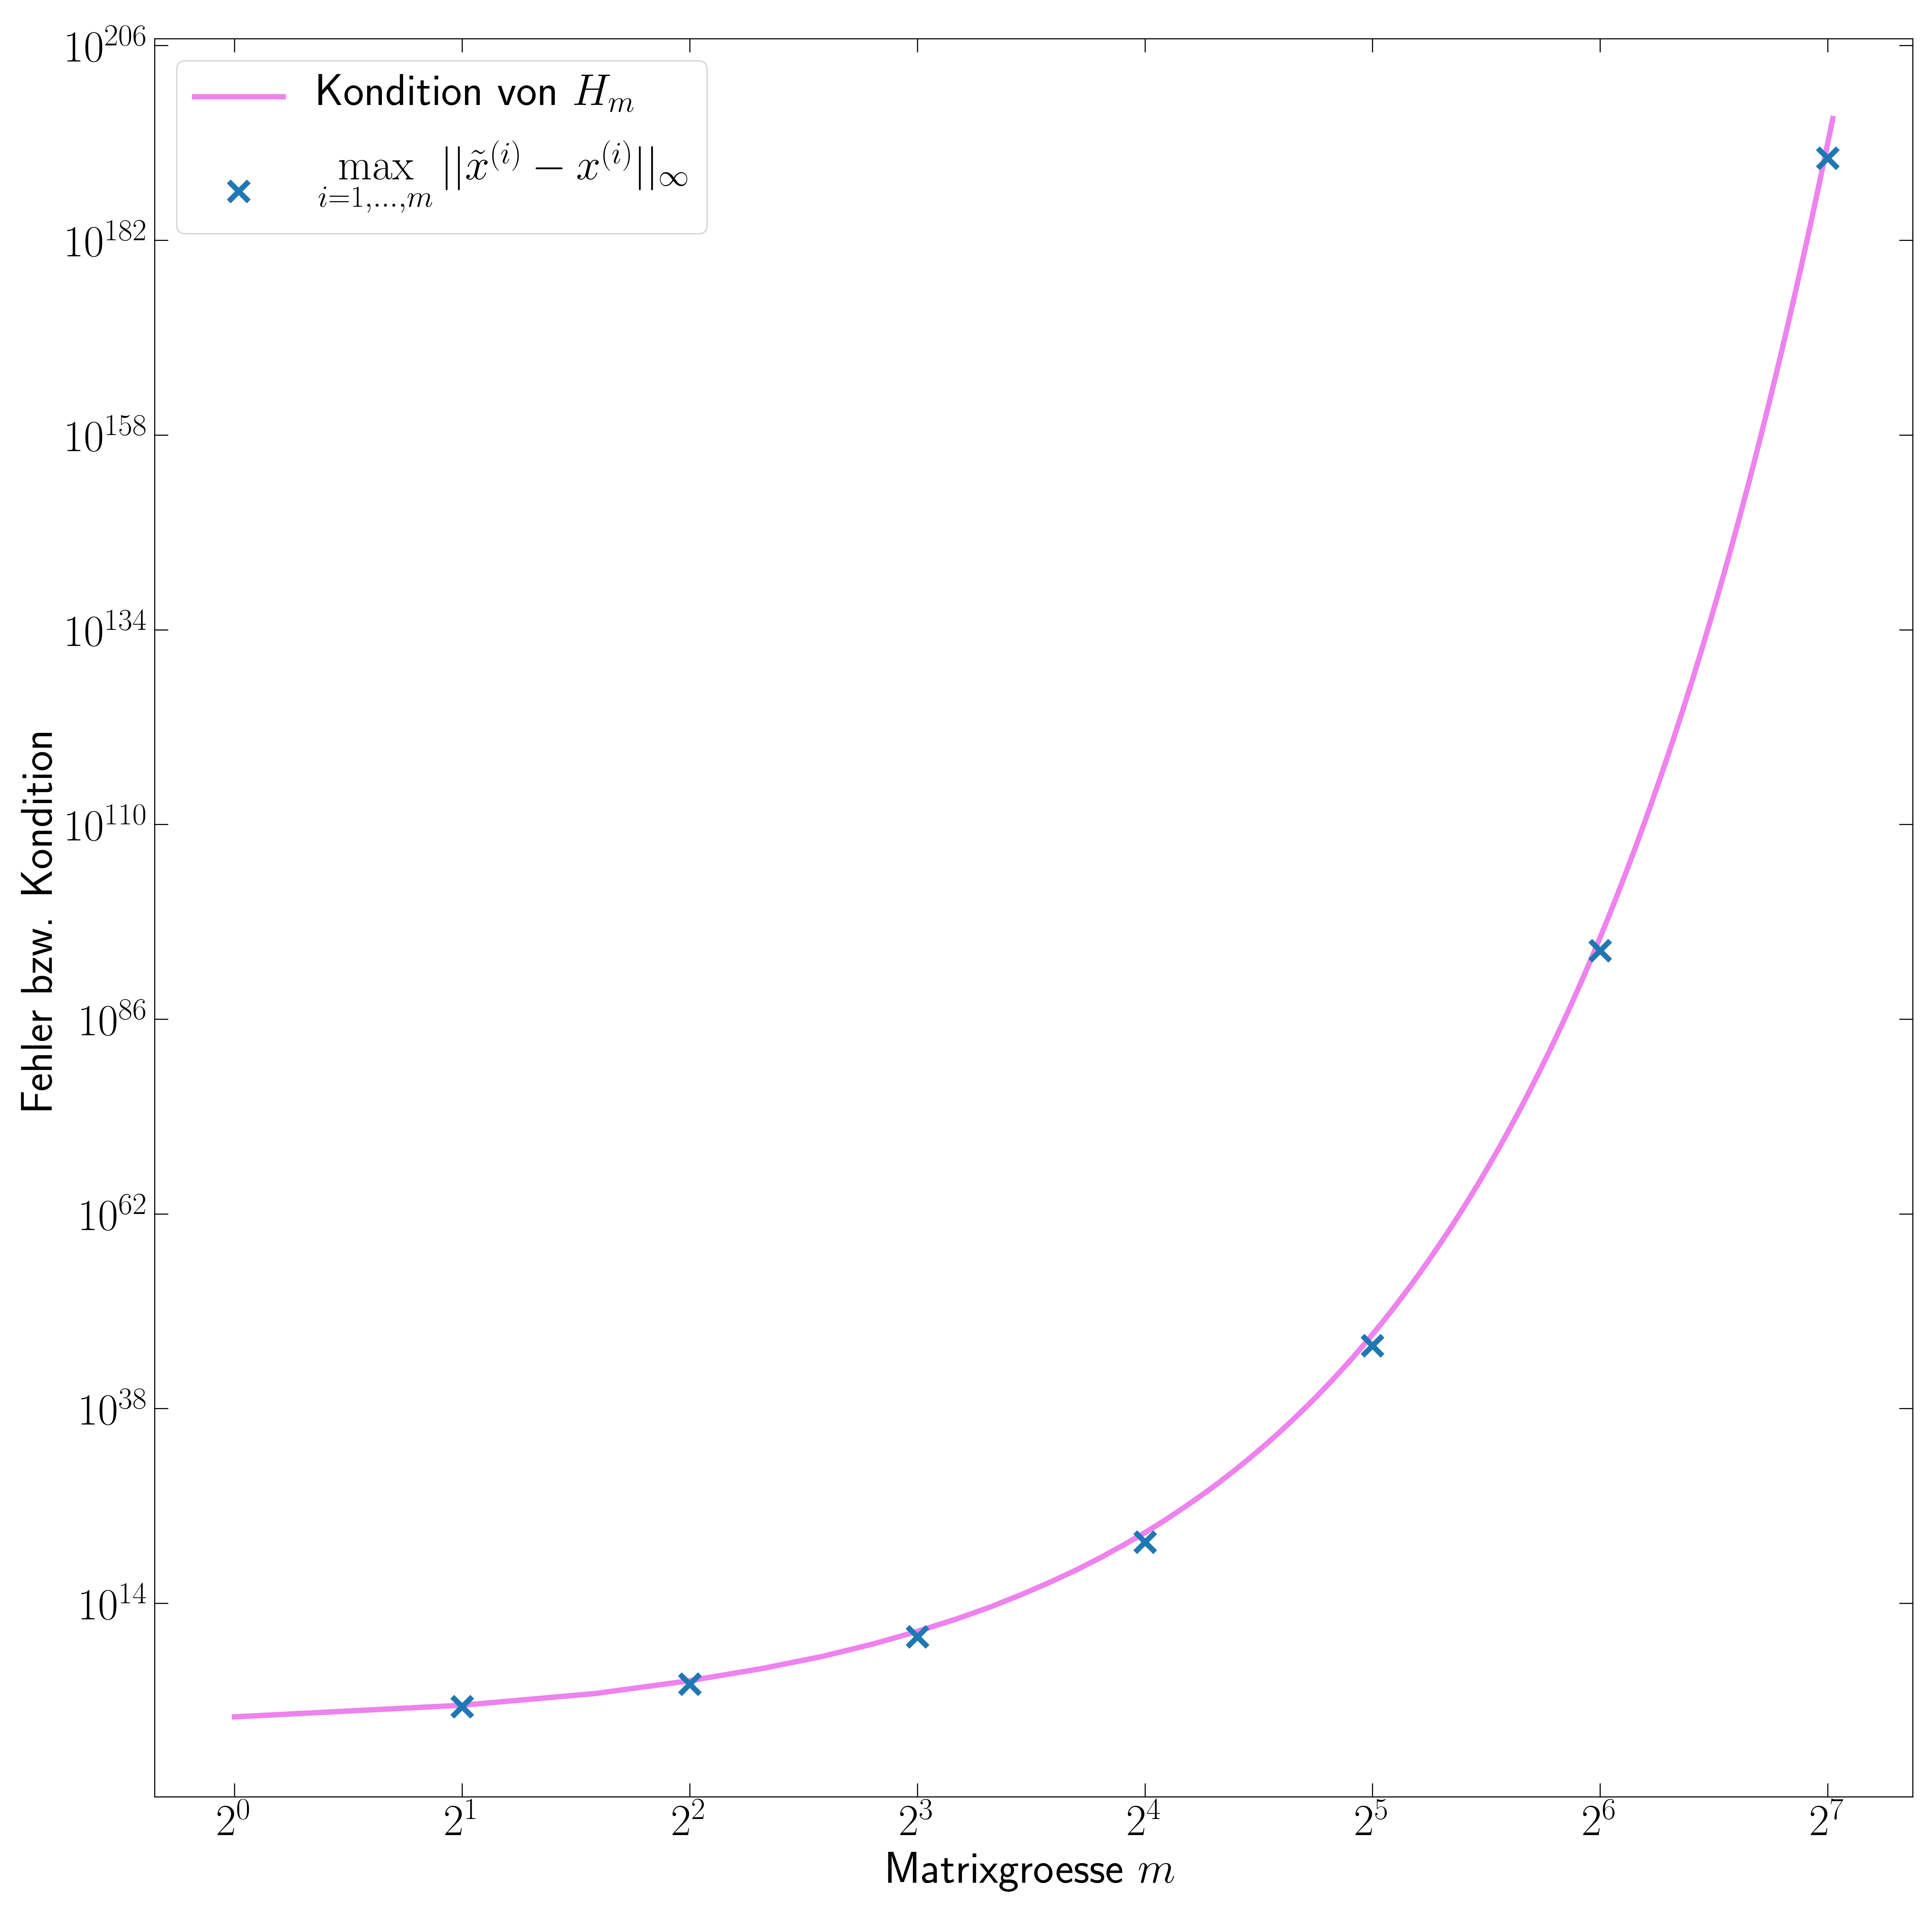
\includegraphics[width=.8\textwidth]{Bericht/Bilder/hil_kond_fehl}
\label{fig:hil_kond_fehl}
\caption{Fehler der numerischen Lösung von \eqref{eq:hil_lgs} und Kondition von $H_m$ in Abhängigkeit von der Matrixgröße $m$.}
\end{figure}

Man erkennt ein starkes Ansteigen der Kondition von $H_m$ mit $m$. $\kappa(H_m)(m)$ ist in der logarithmischen Darstellung im betrachteten Bereich monoton wachsend und konvex, wächst also schneller als jede endliche Potenz von $m$. Der Wert von $\max\|\tilde{x}^{(i)}-x^{(i)}\|_\infty$ ist für die betrachteten $m$ durch $\kappa(H_m)$ beschränkt.

\section{Zusammenfassung}

%TODO NLA Skript zitieren
\begin{thebibliography}{9}
\bibitem{nla} NLA SKRIPT \textit{Sparse Matrix}. 
\url{https://en.wikipedia.org/wiki/Sparse_matrix}
\bibitem{aufg6.2} G. Allaire, S. M. Kaber; Springer Science+Business Media; 2008 \textit{Numerical Linear Algebra}
\url{https://moodle.hu-berlin.de/pluginfile.php/2517254/mod_resource/content/16/Uebungsblatt_06_A2_Loesung.pdf}
\end{thebibliography}


%%% END OF DOCUMENT %%%%%%%%%%%%%%%%%%%%%%%%%%%%%%%%%%%%%%%%%%%%%%%%%%%%%%%%%%%
\end{document}
